\documentclass[10pt,journal,compsoc]{IEEEtran}

\usepackage[all,pdf]{xy}
\usepackage{tikz}

% *** CITATION PACKAGES ***
%
\ifCLASSOPTIONcompsoc
  % IEEE Computer Society needs nocompress option
  % requires cite.sty v4.0 or later (November 2003)
  \usepackage[nocompress]{cite}
\else
  % normal IEEE
  \usepackage{cite}
\fi

% *** MATH PACKAGES ***
%
\usepackage{amsmath}
\usepackage{amsthm}
\usepackage{nicefrac}
\usepackage{array}
\usepackage{lmodern,amssymb}
\usepackage{float}
\usepackage{graphicx}
\usepackage{caption}
\usepackage{subcaption}
\usetikzlibrary{positioning}
\usetikzlibrary{shapes.misc}

\usepackage[utf8]{inputenc}
\usepackage[T1]{fontenc}
\usepackage[english]{babel}
\usepackage{pgfplots}
\usepackage{hyperref}
\usepackage{algorithm}
\usepackage{algpseudocode}

% Commands
\newcommand\smallO{
  \mathchoice
    {{\scriptstyle\mathcal{O}}}% \displaystyle
    {{\scriptstyle\mathcal{O}}}% \textstyle
    {{\scriptscriptstyle\mathcal{O}}}% \scriptstyle
    {\scalebox{.50}{$\scriptscriptstyle\mathcal{O}$}}%\scriptscriptstyle
  }

\interdisplaylinepenalty=2500


\newtheorem{theorem}{Theorem}
\newtheorem{lemma}{Lemma}
\newtheorem{definition}{Definition}

\hyphenation{op-tical net-works semi-conduc-tor}

\DeclareMathOperator{\N}{\mathbb{N}}

\makeatletter
\def\endthebibliography{%
  \def\@noitemerr{\@latex@warning{Empty `thebibliography' environment}}%
  \endlist
}
\makeatother

\begin{document}

\title{Finding Lower Bounds for the Number of Comparisons in Selection Algorithms}
\author{Julius von Smercek, Josua Dörrer, Konrad Gendle, Andreas Steding, Johanna Hofmann% <-this %
  \IEEEcompsocitemizethanks{\IEEEcompsocthanksitem Institut für Formale Methoden der
    Informatik (FMI)\protect\\
    Universität Stuttgart
  }}

\markboth{Bachelor research project}%
{Submission}

\IEEEtitleabstractindextext{%
  \begin{abstract}
    This research project aims to find worst-case optimal comparison algorithms for selecting the $i$-th smallest of $n$ elements in a set for $n$ up to $15$ using computer search.
  \end{abstract}

  \begin{IEEEkeywords}
    Selection, Pessimistic Lower Bound, Partial Order Sets, Computer Search
  \end{IEEEkeywords}}


\maketitle

\IEEEdisplaynontitleabstractindextext


\IEEEpeerreviewmaketitle

\IEEEraisesectionheading{
  \section{Motivation}
  \label{sec:motivation}
} \IEEEPARstart{T}{he} problem of selecting the $i$-th smallest element in a
list of $n$ elements is a well-known problem in computer science called
\textit{selection}. Explicitly, we concern ourselves with the optimal worst-case
selection of a single element from a set of initially unordered unique elements,
measuring the cost as the number of comparisons made. A first approach to solve
this can be achieved by sorting the list at first and selecting the $i$-th
element. However, this approach has a time complexity of $\mathcal{O}(n \cdot
  \log n)$. Putting more thought into this problem one can find algorithms like
the median of medians \cite{Schoening1993} or PICK
\cite{Blum1972} and reduce the time complexity to $\mathcal{O}(n)$.
Optimal algorithms are known for any $n$ when $i$ is either one or two, but
there is a significant performance gap finding the median $i = \nicefrac{n}{2}$
from the best known algorithm with a time complexity of $2.95n$ described in
\cite{dor1999selecting} to the tightest known minimum of $2 \cdot n -
  \smallO(n)$.

Searching for optimal solutions is considerably difficult and the tightest known
lower bounds obtained by mathematical means soon exceed what is attainable by
even rather intelligent search. An approach to finding optimal algorithms is
made by Gasarch, Kelly and Pugh \cite{Gasarch1996} who introduced computer
search to find optimal selection algorithms. On his website Kenneth Oksanen
\cite{Oksanen} published a computer search algorithm improving the previously
known lower bounds found by Gasarch et. al. However, the results are not
published in a scientific journal and lack explanation. This work will continue
the work of Oksanen \cite{Oksanen} by confirming, improving and expanding the
values he found. It will reimplement some ideas of the algorithms Oksanen
published along with his found lower bounds and improve the computer search
algorithms by researching the benefits of different search strategies, adding
$\alpha$-$\beta$-pruning and the exploitation of compatible solutions. A quote
from Miguel de Cervantes from Don Quijote will hold true for this article: The
journey is better than the inn. \cite{cervantes_don_quijote}
So buckle up.

\section{Fundamentals}
\subsection{Algorithms for Finding the $i$-th largest of $n$ elements}
\subsubsection{Sorting}
A baseline algorithm to select the $i$-th element in a list of $n$ values is to
use a sorting algorithm like merge sort or heap sort on the input data and then
return the $i$-th element of the now sorted list. The time complexity of this
approach is essentially the runtime to sort the list. For the sorting algorithms
mentioned the time complexity is of $\mathcal{O}(n \cdot \log n)$

\subsubsection{Pivoting}
A better approach solving the selection problem can be achieved by using
pivoting. The common idea of the algorithms using pivoting is to promote an
element from the input to a so called \textit{pivot} element and use comparisons
against this element to divide the remaining $n - 1$ input elements into two
subsets. Let $L$ be the subset with elements less than the pivot element and $G$
the subset with elements greater than the pivot element. The algorithm can then
determine whether to search for the $i$-th element in the subset $L$ or the
subset $G$. Using pivot algorithms like the quickselect algorithm, the runtime
can be reduced to $\mathcal{O}(n)$.
The first linear-time deterministic selection algorithm known is also commonly
taught in computer science class is the median of medians. It partitions the
input data into sets of five in linear time. Then it calls itself on each of the
sets to find the median of these sets of five. The result is a algorithm that
returns the median in $\mathcal{O}(n)$. In practice the algorithm performs
poorly compared to quickselect and is also slower than sorting the list of
moderate size due to its high constant factor. Better algorithms like
quickselect or PICK have a lower constant factor but all these algorithms share
the same time complexity $\mathcal{O}(n)$. \cite{Blum1972, HoareQuickselect}

\subsubsection{Lower and upper bounds}
The time complexity of $\mathcal{O}(n)$ of the mentioned algorithms is
inevitable, because the input to these algorithm is a list of values in
arbitrary order. Therefore, the algorithm must look at all the input values to
determine a correct solution. If any of these input values will not be
considered it could be the one that should have been returned by the algorithm
leading to wrong results. Apart from this simple and straightforward argument,
there is a considerable amount of research on the exact number of comparisons
required for selection, both in the randomized and deterministic cases.

It has been found that selecting the $i$-th element of $n$ requires at least
$n+\min(i,n-i)-\mathcal{O}(1)$ comparisons \cite{cunto1989}, thus matching the
average case of the Floyd-Rivest algorithm up to its $\smallO(n)$ term. For
deterministic algorithms it has also been shown that
\begin{eqnarray*}
  &\left (1 + H(i/n) \right ) \cdot n + \Omega(\sqrt n) \\
  &\text{with~} H(x) = x \cdot \log_2 \frac{1}{x} + (1-x) \log_2 \frac{1}{1-x}
\end{eqnarray*}
comparisons are required. An upper bound is been proposed by Blum, in the paper
\textit{Time Bounds for Selection}. \cite{Blum1972} It stated that no more than
$5.430\dot{5} \cdot n$ comparisons are ever required. \cite{Blum1972} Therefore
selection is for sure in a time complexity of $\mathcal{O}(n)$ for best and
worst-case.

\begin{lemma} \label{lemma:previous_next_poset}
  If $k$ is a lower bound for selecting $i$ of $n$, then selecting $i$ of $n + 1$ must take at least $k + 1$ comparisons.
\end{lemma}

\begin{proof}
  Assume some algorithm exists that selects $i$ of $n + 1$ in $k$ comparisons.
  It must have two elements it compares first.
  If we input a by definition largest element in place of one of them the algorithm must still return the correct $i$-th largest of the remaining $n$ elements.
  But because this element is larger by definition, the first comparison may be skipped, thus reducing the number of comparisons by at least $1$.
  Thus taking out all occurrences of that element will yield an algorithm for $i$ of $n$ in $k - 1$ comparisons, which contradicts the condition of $k$ being a lower bound.
\end{proof}

\subsection{Partial Order Sets}
To dive deeper into these algorithms the concept of partial orders needs to be introduced.
A partial order is an ordering relation $\leq$ on a set $P$ that satisfies reflexivity, antisymmetrie, and transitivity.
Furthermore, we assume in the following that all numbers are pairwise different.

\begin{definition}[Selection poset]
  Given a set of elements $\Omega$ with $|\Omega| = n < \infty$ we write $(n, i, R)$ for the selection of the $i$-th largest of $n$ elements with the existing comparisons $R$.
  Explicitly, $R\subseteq\Omega^2$ such that $(a, b)\in R \Longleftrightarrow a \leq b$.

  The enumeration of $i$ starts at $0$, so in $(4, 1, R)$ is the second smallest searched, rather than the minimum.
\end{definition}

The select problem is thus embedded as $(n, i, \emptyset)$.

\begin{definition}[Dual poset] \label{definition:dual_poset}
  The dual of a poset $P = (n, i, R)$ is the poset $P^{-1} = (n, n - 1 - i, R')$ with $R' = \{(u,v) \mid (v,u) \in R\}$.
\end{definition}

\begin{definition}[Reduced] \label{definition:reduced_poset}
  A poset is \textbf{reduced} if all its elements have at most $i$ elements smaller than themselves and at most $n - 1 - i$ larger than themselves.
  Hence, all elements are still possible solutions.
\end{definition}

\begin{definition}[Canonified]
  A poset is \textbf{canonified} if it matches the following conditions making it unique among all posets isomorphic to it:
  \begin{itemize}
    \item all elements in the poset are arranged canonically, i.e. all permutations of these elements must map to this poset
    \item
          If $i = n - 1 - i$ applies, the dual poset is formed, both are canonified and deterministically decided which of the two posets corresponds to the canonified representation.
          This is also described in more detail in Section~\ref{sec:backward:normal_form}
  \end{itemize}

  Some parts of this paper use a best effort approximation for this to increase speed, the results are then called \textbf{pseudo canonified}.
\end{definition}

\begin{definition}[Normal]
  A \textbf{normal} poset is reduced and canonified.
\end{definition}

\begin{definition}[Optimal Cost]
  The cost $V(P)$ of the poset $P = (n, i, R)$ is the optimal number of further comparisons needed to perform the selection.

  We measure this pessimistically, meaning that among all possible outcomes of those further comparisons we assume the most expensive ones.
\end{definition}

\begin{lemma} \label{lemma:dual_poset_allowed}
  For a given poset $P = (n, i, R)$ it holds $V(P) = V(P^{-1})$
\end{lemma}

\begin{proof}
  Given $V(P)$, we know that we can construct an algorithm that solves $P$ in exactly that many comparisons, i.e. it determines the element with exactly $i - 1$ less and exactly $n - i$ greater than itself.

  Since $n$ and $i$ are fixed, this algorithm can be converted into a binary decision tree and by swapping all the children, the new algorithm must now select the element such that $n - i$ are smaller and $i - 1$ are larger than it while assuming an inverted $R$, which is the solution for $P^{-1}$.
\end{proof}


\subsubsection{Solved posets and Compatible Solutions}
By definition of the problem, we seek an element that is larger than $n-i$ elements and smaller than $i - 1$ elements.

\begin{lemma}\label{lemma:partition}
  Solving a poset requires knowing the explicit elements making up these two sets.
\end{lemma}

\begin{proof}
  Suppose we have determined the element $e$ to be the solution, and an element $p$ unordered with $e$.

  Then $p$ may be above as well as below $e$, which can't be the solution in both cases.
\end{proof}

\begin{definition}[Compatible Solution]
  As such we can define a \textbf{compatible solution} $Q = (n, i, S)$ of a poset $P = (n, i, R)$, to be solved and agreeing with $P$, that is $(a, b)\in S\implies (b, a)\notin R$.

  Furthermore, $Q$ has no comparisons other than the $n - 1$ needed to prove the solution and the ones resulting from application of transitivity to the former.
\end{definition}

With Lemma~\ref{lemma:partition}, a solved poset has exactly one compatible solution.

Let $\mathcal{C}(P) = \{Q \mid Q \text{ compatible with } P\}$ be the set of all solutions compatible with $P$.

\begin{lemma}\label{lemma:compatible_union}
  For a poset $P = (n, i, R)$ and $a, b$ with $(a, b), (b, a)\notin R$ it holds $\mathcal{C}(P) = \mathcal{C}(n, i, R \, \cup \{(a, b)\}) \cup \mathcal{C}(n, i, R\cup \{(b, a)\})$.
\end{lemma}

\begin{proof}
  Let $Q = (n, i, S)\in \mathcal{C}(P)$.
  Then for all $c, d$ other than $a, b$ it must hold that $(c, d)\in S\implies (d,c)\notin R\cup \{(a, b)\}$ and $(c, d)\in S\implies (d, c)\notin R\cup \{(b, c)\}$.

  So if $(a, b)\in S$ then $Q\in\mathcal{C}(n, i, R\cup \{(a, b)\})$, if $(b, a)\in S$ then $Q\in\mathcal{C}(n, i, R\cup \{(b, a)\})$
  and if $a, b$ are unordered in $Q$, it is in both.

  The reverse also holds because $(c, d)\notin R\cup \{(a, b)\}\implies (c, d)\notin R$, same for $R\cup \{(b, a)\}$.
\end{proof}

\begin{theorem}\label{theorem:compatible_log}
  A poset $P=(n,i,R)$ cannot be solvable in less than $\lceil\log_2(|\mathcal{C}(P)|)\rceil$ comparisons in the worst case.
\end{theorem}

\begin{proof}
  If $P$ is already solved, $|\mathcal{C}(P)|=1$, and $\log_2(1)=0$.

  If not, we must make at least one more comparison $a, b$.

  From Lemma~\ref{lemma:compatible_union} we also know that
  $$|\mathcal{C}(P)| \leq |\mathcal{C}((n,i,R\cup \{(a, b)\}))| + |\mathcal{C}((n,i,R\cup \{(b, a)\}))|$$

  Since this is a pessimistic measure, we must assume that the result of the comparison results in the one with more compatible solutions.
  Without loss of generality we assume that to be $(a, b)$.
  Then

  $$\frac{|\mathcal{C}(P)|}{2}\leq |\mathcal{C}((n,i,R\cup \{(a, b)\}))|$$

  Repeated application of this over multiple comparisons results in $\frac{|\mathcal{C}(P)|}{2^j}$ as the lower bound for the amount of compatible solutions after $j$ comparisons.

  Since $|\mathcal{C}(P)|\leq 2^j$ must be satisfied for the solution, $j\geq\log_2(|\mathcal{C}(P)|)$
\end{proof}


\subsection{Example}
\begin{figure}[!b]
  \centering
  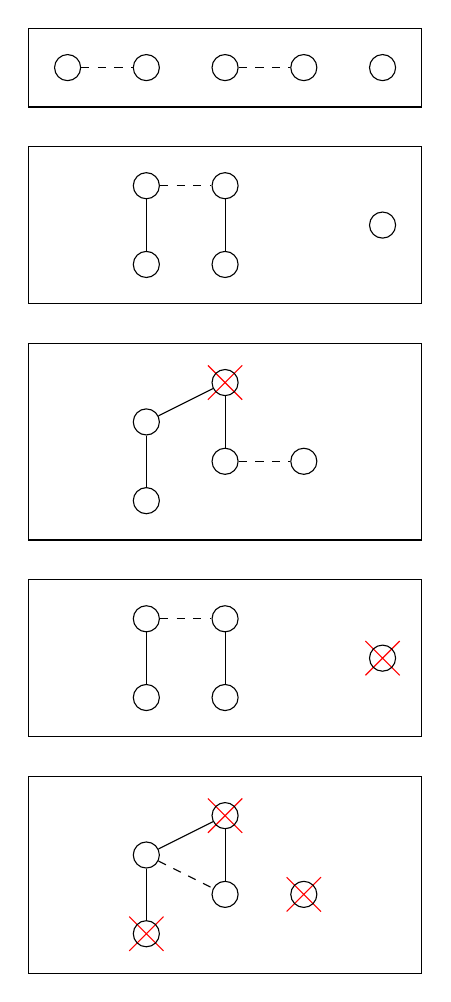
\begin{tikzpicture}[tcancel/.append style={draw=#1, cross out, inner sep=6pt}]
  \draw(-.5, -.5) rectangle (4.5, .5);
  \node[circle,draw=black] (A1) at (0, 0) {};
  \node[circle,draw=black] (A2) at (1, 0) {};
  \node[circle,draw=black] (A3) at (2, 0) {};
  \node[circle,draw=black] (A4) at (3, 0) {};
  \node[circle,draw=black] (A5) at (4, 0) {};

  \draw[dashed] (A1) -- (A2) node {};
  \draw[dashed] (A3) -- (A4) node {};

  \draw(-0.5, -3.0) rectangle (4.5, -1.0);
  \node[circle,draw=black] (B1) at (1.0, 0 - 2.5) {};
  \node[circle,draw=black] (B2) at (1.0, 1 - 2.5) {};
  \node[circle,draw=black] (B3) at (2.0, 0 - 2.5) {};
  \node[circle,draw=black] (B4) at (2.0, 1 - 2.5) {};
  \node[circle,draw=black] (B5) at (4.0, 0.5 - 2.5) {};

  \draw (B1) -- (B2) node {};
  \draw (B3) -- (B4) node {};
  \draw[dashed] (B2) -- (B4) node {};

  \draw(-0.5, -6.0) rectangle (4.5, -3.5);
  \node[circle,draw=black] (C1) at (1, 0 - 5.5) {};
  \node[circle,draw=black] (C2) at (1, 1 - 5.5) {};
  \node[circle,draw=black,tcancel=red] (C3) at (2, 1.5 - 5.5) {};
  \node[circle,draw=black] (C3) at (2, 1.5 - 5.5) {};
  \node[circle,draw=black] (C4) at (2, .5 - 5.5) {};
  \node[circle,draw=black] (C5) at (3, .5 - 5.5) {};

  \draw (C1) -- (C2) node {};
  \draw (C3) -- (C4) node {};
  \draw (C2) -- (C3) node {};
  \draw[dashed] (C4) -- (C5) node {};

  \draw(-0.5, -8.5) rectangle (4.5, -6.5);
  \node[circle,draw=black] (D1) at (1.0, 0 - 8) {};
  \node[circle,draw=black] (D2) at (1.0, 1 - 8) {};
  \node[circle,draw=black] (D3) at (2.0, 0 - 8) {};
  \node[circle,draw=black] (D4) at (2.0, 1 - 8) {};
  \node[circle,draw=black,tcancel=red] (D5) at (4.0, 0.5 - 8) {};
  \node[circle,draw=black] (D5) at (4.0, 0.5 - 8) {};

  \draw (D1) -- (D2) node {};
  \draw (D3) -- (D4) node {};
  \draw[dashed] (D2) -- (D4) node {};

  \draw(-0.5, -11.5) rectangle (4.5, -9.);
  \node[circle,draw=black,tcancel=red] (E1) at (1, 0 - 11.0) {};
  \node[circle,draw=black] (E1) at (1, 0 - 11.0) {};
  \node[circle,draw=black] (E2) at (1, 1 - 11.0) {};
  \node[circle,draw=black,tcancel=red] (E3) at (2, 1.5 - 11.0) {};
  \node[circle,draw=black] (E3) at (2, 1.5 - 11.0) {};
  \node[circle,draw=black] (E4) at (2, .5 - 11.0) {};
  \node[circle,draw=black,tcancel=red] (E5) at (3, .5 - 11.0) {};
  \node[circle,draw=black] (E5) at (3, .5 - 11.0) {};

  \draw (E1) -- (E2) node {};
  \draw (E3) -- (E4) node {};
  \draw (E2) -- (E3) node {};
  \draw[dashed] (E2) -- (E4) node {};
\end{tikzpicture}
  \caption{Finding the median $i = 2$ of $n = 5$ values using six comparisons.}
  \label{fig:median_of_5}
\end{figure}
A good visual example is finding the median $i=2$ in a list of $n = 5$ elements.
Figure~\ref{fig:median_of_5} illustrate the search of the median using Hasse diagrams.
Each step shows the comparisons to be performed next as a dashed line.
A Hasse diagram of the order of relation found so far (smaller=lower, larger=higher) is shown as the solid lines.
The red crosses indicate elements that have been found to be greater or smaller than three other elements and therefore are disqualified for the median.
The larger element of the final comparison is the median.
This is also the optimal algorithm for $i = 2$ and $n = 5$.


\section{Methods and Tools}
In this section we describe our three main approaches being the forward search, backward search and bidirectional search.
Furthermore, we explain how we harness the notion of compatible solutions with respect to all of the three search approaches.

\subsection{Forward Search}\label{chapter:forward_search}
Forward search starts with an unordered poset $P=(n,i,\emptyset)$, and recursively determines solvability of a given poset within some bound by exhaustively searching the results of all possible comparisons to be made unless it is already solved or we determine that it cannot be solved within the alloted number of comparisons by some solvability-check.

Between the two possible outcomes of a comparison we assume the worse, but since an algorithm is free to choose which elements to compare we are looking for the most useful comparison, the one that yields result posets cheapest to solve themselves, still in terms of worst case outcome.
The algorithms output by the search program are built by saving the comparison that lead to this cheapest to solve result.

To limit memory cost and allow further pruning we traverse the search tree depth first, reducing the maximum number of comparisons alloted to child posets to one less than the current best result found.
This premise is implemented by Minimax algorithms as shown in Figure~\ref{fig:minimax_search}.

We can drastically speed up this exploration by caching previous results, even with a simple usage based ejection policy. Since the search always imposes an upper bound for the number of comparisons to allow this also includes yet unsolved posets, for which we note the currently known minimum.

\subsubsection{Pruning Decisions}
The minimax search algorithm allows for cutting off unpromising branches.
For this means, the following strategies are applied.

\begin{enumerate}
  \item[1.]
    Use solvability-check. For an unsolvable poset the check always returns 'unsolvable'.
    However, the check may return 'solvable' or 'unsolvable' for a poset that is in fact solvable.
    If the check returns 'unsolvable', the branch is pruned.
    Otherwise, the search is continued in the current branch.
  \item[2.]
    Use \texttt{current\_best}. This variable facilitates cutting off branches according to the idea of alpha-beta pruning.
\end{enumerate}

It is optimal because of an inductive argument over the number of relative orders determined.
An already solved poset obviously takes no further comparisons to solve.
Then, given an unsolved poset with all elements already too large or small excluded we must make at least one more comparison to
make progress.
Since all posets resulting from these comparisons must have more elements ordered than the current one has we can assume as per induction that we know their optimal cost.
As a result, we cannot solve the poset in less than the cost of the cheapest of these comparisons, plus one for the comparison itself, hence the current poset is also solved optimally.

It is also complete for a given upper bound, explainable through a similar inductive argument.
If the poset is solvable within that bound, then at least one of its possible comparisons must have both outcomes be solvable within the bound lowered by one.
Since the search only lowers the bound imposed on its recursive descendants beyond that once at least one has been solved, we are also guaranteed to find a solution for the original poset if it exists within the bound.

\begin{figure}[!b]
  \centering
  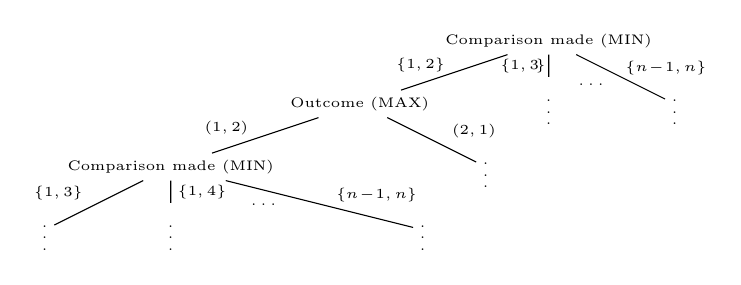
\begin{tikzpicture}[scale=0.8]
  \tiny
  \node (A1) at (0,0) {$\vdots$};
  \node (A2) at (2,0) {$\vdots$};
  \node (A3) at (3.5,0.4) {$\dots$};
  \node (A4) at (6,0) {$\vdots$};

  \node (B1) at (2,1) {Comparison made (MIN)};

  \draw (B1) -- (A1) node[above,pos=0.6, xshift=-0.4cm] {$\{1,3\}$};
  \draw (B1) -- (A2) node[right, midway] {$\{1,4\}$};
  \draw (B1) -- (A4) node[right, pos=0.3, xshift=6mm] {$\{n \!- \! 1,n\}$};

  \node (C1) at (5,2) {Outcome (MAX)};
  \node (B2) at (7,1) {$\vdots$};

  \draw (C1) -- (B2) node[right, pos=0.3, xshift=4mm] {$(2,1)$};

  \draw (B1) -- (C1) node[left, pos=0.7, xshift=-4mm] {$(1,2)$};

  \node (D1) at (8,3) {Comparison made (MIN)};
  \node (C2) at (8,2) {$\vdots$};
  \node (C3) at (8.7,2.3) {$\dots$};
  \node (C4) at (10,2) {$\vdots$};

  \draw (D1) -- (C1) node[left,pos=0.3,xshift=-3mm] {$\{1,2\}$};
  \draw (D1) -- (C2) node[left, midway, xshift=0.5mm] {$\{1,3 \! \}$};
  \draw (D1) -- (C4) node[right, pos=0.3,xshift=2mm] {$\{n \! - \! 1,n\}$};

\end{tikzpicture}
  \caption{Minimax search algorithm}
  \label{fig:minimax_search}
\end{figure}

\subsubsection{Canonification}

When caching the posets we have to check whether two posets are isomorphic to each other.
We consider a poset isomorphic to another poset if we can relabel the elements of one poset to obtain the other poset.
This problem is expensive to solve for every poset comparison.

After adding a comparison to a poset, we transform the poset to a canonical form.
All posets, that are isomorphic to each other should be transformed to the same canonical form.
Computing the canonical form can be done using Nauty, but this takes a significant amount of time.
Some performance tests show that it is faster to compute an almost canonical form, where some posets that are isomorphic to each other result in different canonified forms.
As a result, some posets that are isomorphic occupy several cache entries, but canonifying a poset is much faster.

\subsubsection{Heuristics}

We used multiple heuristics to estimate if a poset is solvable in a given number of comparisons.
These heuristics are used to reject posets that are not solvable in the given number of comparisons.
Other than caching, no strategies to preemptively prove solvability within some bound were employed.
This means that the following heuristics must only provably be not too pessimistic.

The first heuristic uses the number of compatible solutions.
We use the fact, proven in Theorem \ref{theorem:compatible_log}, that the $\log_2$ of the number of compatible solutions is a lower bound for the cost of a poset.

Algorithm~\ref{algo:compatible_solutions} shows an algorithm for computing the number of compatible solutions for a poset.
The algorithm assumes that the elements in the poset are sorted in such a way that an element that is smaller than another has a smaller index.
The calculation of this number first picks a solution element $j$ - since posets are always reduced in the forward search any element is valid - and then counts the number of possible separations into greater and lesser elements, summing up these counts over all solution elements.

\begin{algorithm}[t]
  \centering
  \begin{algorithmic}

    \Function{NumCompatibleSolutions}{$(P, i)$}

    \State{$c \gets 0$}

    \For{$j \in \Omega_P$} \Comment{solutions with $j$ $i$-th smallest}

    \State{$\mathcal{D} \gets \{ \less{P}{j} \setminus \{j\} \}$}% \Comment{downsets containing $\less{P}{j} \setminus \{j\}$}

    \For{$k \in \Omega_P \setminus (\less{P}{j} \cup \greater{P}{j})$}

    \For{$S \in \mathcal{D}$}

    \If{$\less{P}{k} \subseteq S \cup \{ k \}$}
    \State{$\mathcal{D} \gets \mathcal{D} \cup \{ S \cup \{ k \} \}$}
    \EndIf

    \EndFor

    \EndFor

    \State{$c \gets c + |\{S \in \mathcal{D} \mid |S| = i \}|$}

    \EndFor

    \State{\Return{$c$}}

    \EndFunction
\end{algorithmic}

% New Version

% pub fn num_compatible_posets(&self) -> usize {
% debug_assert!(self.is_lower_triangle_matrix());

% let all_less_than = {
%     let mut bitsets = [BitSet::empty(); MAX_N];
%     bitsets
%         .iter_mut()
%         .take(self.n() as usize)
%         .enumerate()
%         .for_each(|(i, bs)| *bs = self.get_all_less_than(i as u8));
%     bitsets
% };

% let mut less_subsets = Vec::with_capacity(1000);

% let mut sum = 0;
% for i in 0..self.n() as usize {
%     // assume the ith element is the solution

%     let less_than_i = all_less_than[i];

%     if less_than_i.len() == self.i() as usize {
%         sum += 1;
%         continue;
%     }
%     if less_than_i.len() > self.i() as usize {
%         continue;
%     }

%     let greater_than_i = self.get_all_greater_than(i as u8);
%     let ordered_with_i = less_than_i.union(greater_than_i);

%     less_subsets.clear();
%     less_subsets.push(less_than_i);

%     for j in 0..self.n() as usize {
%         if j == i || ordered_with_i.contains(j) {
%             continue;
%         }

%         let less_than_j = all_less_than[j];

%         // try adding j to all previous subsets
%         for i in 0..less_subsets.len() {
%             let subset = less_subsets[i];

%             // test if adding j would make a valid subset
%             // we know, that there is no k with p[k] > p[j]
%             if less_than_j.intersect(subset) == less_than_j {
%                 let mut new_subset = subset;
%                 new_subset.insert(j);
%                 less_subsets.push(new_subset);
%             }
%         }
%     }

%     sum += less_subsets
%         .iter()
%         .filter(|s| s.len() == self.i() as usize)
%         .count();
% }

% sum
% }

% Old Version

% pub fn num_compatible_posets(&self) -> usize {
%     let canonified = self.canonify_lower_matrix();

%     let mut sum = 0;
%     for i in 0..canonified.n {
%         // assume the ith element is the solution

%         let less_than_i = canonified.get_all_less_than(i);
%         let greater_than_i = canonified.get_all_greater_than(i);

%         let mut less_subsets = Vec::new();
%         less_subsets.push(BitSet::empty());

%         for j in 0..canonified.n {
%             if j == i || greater_than_i.contains(j as usize) {
%                 continue;
%             }

%             let less_than_j = canonified.get_all_less_than(j);

%             // try adding j to all previous subsets
%             if less_than_i.contains(j as usize) {
%                 // all subsets must contain j to be valid

%                 let mut next_free = 0;
%                 for i in 0..less_subsets.len() {
%                     let subset = less_subsets[i];

%                     // test if adding j would make a valid subset
%                     // we know, that there is no k with p[k] > p[j]
%                     if less_than_j.intersect(subset) == less_than_j {
%                         let mut new_subset = subset;
%                         new_subset.insert(j as usize);
%                         less_subsets[next_free] = new_subset;
%                         next_free += 1;
%                     }
%                 }
%                 less_subsets.truncate(next_free);
%             } else {
%                 for i in 0..less_subsets.len() {
%                     let subset = less_subsets[i];

%                     // test if adding j would make a valid subset
%                     // we know, that there is no k with p[k] > p[j]
%                     if less_than_j.intersect(subset) == less_than_j {
%                         let mut new_subset = subset;
%                         new_subset.insert(j as usize);
%                         less_subsets.push(new_subset);
%                     }
%                 }
%             }
%         }

%         sum += less_subsets
%             .into_iter()
%             .filter(|s| s.len() == canonified.i as usize)
%             .count();
%     }

%     sum
% }
  \caption{An algorithm for computing the number of compatible solutions for a given poset.}
  \label{algo:compatible_solutions}
\end{algorithm}

As an example, the unordered poset $(n,i,\emptyset)$ has $n \cdot \binom{n - 1}{i}$ compatible solutions because
for each of the $n$ elements, all separations of the remaining $n - 1$ elements
are valid.


The second heuristic attempts to reduce the size of the searched subtree by adding a `useful' comparison to eliminate elements faster.
Explicitly, it searches for unordered elements $i$ and $j$ such that $i$ has as many elements less than it as possible and $j$ as many as possible greater and adds $i < j$ to the poset.
If there is no $i$ with at least two elements less than it or no $j$ with at least 2 greater, the algorithm aborts the heuristic and resumes regular search.
Otherwise, the new poset is then searched for a solution using the forward search described above without reducing the number of allowed comparisons.
If the new poset is found to be solvable in the given number of comparisons, we estimate that the original poset is also solvable.
If the new poset is not solvable, we estimate the original is not solvable either.
This heuristic can be slightly improved by maximizing the number of elements smaller than the maximal element and greater than the minimal element.
This is admissible because having a comparison added `for free' does not make the poset harder to solve.

\subsubsection{Triangular Adjacency Matrix}
Storing an adjacency matrix for a poset of size $n$ takes $n^2 - n$ bits, one for each possible relation.
The diagonal does not need to be stored, as an element can not be smaller than itself.

By canonifying the poset, the elements can be sorted in a way such that each element is not smaller than any element before it.
This property can be used to reduce the adjacency matrix to a triangular matrix, which can then be stored using $\frac{n^2 - n}{2}$ bits.
It can also simplify some algorithms, for example calculating the number of compatible solutions.

\subsubsection{Multithreading}

Since the forward search recursively explores posets, it is possible to treat subtrees as separate tasks and run them on multiple threads.
We chose to give the thus far implicit search tree an explicit tree structure keeping track of the given poset for later caching, the current best result and number of open child tasks.

Additionally, the tasks also save the second poset of the two outcomes of a comparison to avoid having to maintain separate
MIN and MAX nodes. Once the first poset completes with a better result, the task replaces itself with that for the second poset and expands again.

Unexpanded tasks are pushed into a shared task heap ordered first by number of remaining comparisons to limit breadth-first expansion and thus size of the search tree, then by the number of compatible solutions.
An observation from single threaded runs that completed quickly after the first few posets of depth around $6$ were done also led us to prevent multithreading above that depth by keeping the respective posets in a separate queue.

While this resulted in good speedup for the early iterative deepening runs, it became worse as the search approached the actually required number of comparisons.
For some this was even worse than single threaded search at a noticeably higher cache usage, leading us to ultimately abandon multithreading and calculate the final numbers for $n = 15$ using a single core.

We assume that the heap approach potentially buries promising paths from completely being searched, preventing propagation of the results and thus the pruning exploitation of a found best from reducing the search tree size so often in later runs that the increased workload overtakes the core utilization boost.

See the git branch \textit{multi-threaded} for the last state.

\subsection{Backward Search} \label{sec:backward}

\subsubsection{Idea}

To develop the backward search, primarily the backward search from \cite{stober2022lower} was taken as orientation, since it represents a new research area for the selection problem and was not addressed in the previous work by Oksanen \cite{Oksanen}.

The backward search starts with the solved poset and iteratively removes comparisons until the searched poset is found.
It should be noted that if a comparison is removed from the poset $P = (n, i, R)$ resulting in the poset $P' = (n, i, R \setminus (u, v))$,
the poset $Q = (n, i, R \setminus (u, v) \cup (v, u))$ should already be in a canonified from in the cache.
This means that $Q$ has already been discovered in the search.

Thus, the number of iterations taken until a poset is added to the cache equals the number of worst case comparisons needed to solve it, which means that the search terminates once $(n, i, \emptyset)$ with the desired $n$ and $i$ is found.

% The argument for correctness is that the number of comparisons for which we have found all posets solvable within them equals the number of iterations of the search.
% If for a given poset and a comparison within it we have already discovered both results then their cost must be less than the current number of iterations.
% Hence, we can conclude that the poset is solvable within this number of comparisons.
% Since this condition did not hold true in any previous iteration, we can further infer that the cost must also be optimal.
% And if a poset is solvable within that number of comparisons it must have at least one comparison with a result among the posets discovered in the previous iteration, as otherwise it would have to be solvable in less.


\subsubsection{Algorithm} \label{sec:backward:algorithm}
The input parameters for the backward search are denoted by $n$ and $i$, like in the forward search.
The backward search starts with the smallest solved poset $P_{\text{unordered} (1, 0)} = (1, 0, \emptyset)$ and iteratively computes all posets solvable within $k = 1, 2, 3, \dots$ comparisons until the unordered poset $P_{\text{unordered} (n, i)} = (n, i, \emptyset)$ is encountered.

Let $A_k$ denote the set of all posets solvable in $k$ comparisons.
For all $n$ and $i$, we have $A_0 = { (1, 0, \emptyset) }$.

The backward search begins with $A_0$ and iteratively computes, for each poset in the set $A_k$, the corresponding predecessors, which form the set $A_{k + 1}$.
If $(n, i, \emptyset) \in A_l$, then $l$ comparisons are the lower bound to determine the $i$-th smallest element of an $n$-element list.


\subsubsection{Predecessor calculation} \label{sec:backward:predecessor_calculation}

\begin{definition}[Predecessor] \label{definition:predecessor_calculation}
  Poset $Q$ is the predecessor of poset $P$ if the following conditions hold:
  \begin{itemize}
    \item poset $P$ and $Q$ are both normalized
    \item poset $Q$ was not found in any previous round (otherwise it would be solvable in fewer comparisons)
    \item There exists a comparison $(i, j)$ whose adding in $Q$ and subsequent normalization results in the poset $P$ and adding the reverse comparison $(j, i)$ and subsequent normalization results in an already found poset
  \end{itemize}
\end{definition}

\begin{lemma} \label{lemma:predecessor_calculation}
  If poset $P$ is solvable in $k$ comparisons and $Q$ is a predecessor of poset $P$, poset $Q$ is solvable in $k + 1$ comparisons.
\end{lemma}

\begin{proof} \label{proof:predecessor_calculation}
  Since $Q$ was not found in any previous round, according to the assumption, it is not solvable in fewer comparisons.
  By performing the addition of comparison $(i, j)$ followed by normalization, the poset $P$ is derived, consequently establishing the reachability of $Q$.
  As $P$ is solvable in $k$ comparisons, thus $Q$ is solvable in $k + 1$ comparisons.
  If the comparison is inserted in reverse, according to the assumption, the resulting poset is already in the cache.
  Thus, this path is solvable in at most $k + 1$ comparisons.
\end{proof}

In the following, it is shown how a predecessor is calculated for a given poset $P = (n_P, i_P, R_P)$. As there are potentially many predecessors that cannot contribute to the solution, they are only calculated up to a maximum limit of $n_P$ elements. This is possible because a predecessor always has more or the same number of elements.

Furthermore, not all predecessors are calculated, as some cannot contribute to a solution.
As illustrated in Table~\ref{table:n_i_values_calculated}, the search with $n = 7$ and $i = 3$ only considers predecessors that have an `x' in the corresponding row or column. As the addition of a comparison can reduce $n$ by a maximum of $1$ and therefore $i$ by a maximum of $1$, all other predecessors can be ignored as they can never be used.
For example, no poset with $n = 6$ and $i = 1$ can result in a poset of size $n = 7, i = 3$ by adding a comparison.

The table can be calculated by marking initial $n, i$ with an `x' and then marking recursive the entries for $n - 1, i$ and $n - 1, i - 1$ with an `x', as in each step the new element could be smaller or larger than the i-smallest element.

For Table~\ref{table:n_i_values_calculated}, this means that $n = 6, i = 2$ and $n = 6, i = 3$ should be marked.
It must be noted that $n = 6, i = 3$ does not exist, as the dual poset would be formed at this point.
In this case, only $n = 6, i = 2$ is marked with an `x'.

\begin{table}[!t]
  \renewcommand{\arraystretch}{1.2}
  \caption{Possible predecessors that must be calculated for $n = 7$ and $i = 3$. All predecessors for which the corresponding field is marked with `x' must be calculated.}
  \label{table:n_i_values_calculated}
  \centering
  \begin{tabular}{c|cccc}
    $n$ & \multicolumn{4}{c}{$i$}             \\
        & 0                       & 1 & 2 & 3 \\ \hline
    7   & -                       & - & - & x \\
    6   & -                       & - & x & - \\
    5   & -                       & x & x & - \\
    4   & x                       & x & - & - \\
    3   & x                       & x & - & - \\
    2   & x                       & - & - & - \\
    1   & x                       & - & - & - \\
  \end{tabular}%
\end{table}

The computation of a predecessor for a given poset $P = (n_P, i_P, R_P)$ proceeds in four steps:

\begin{itemize}
  \item[1.]
    First, we search for all posets with $n_P$ elements that result in poset $P$ after inserting a comparison $u < v$ and then canonifying it.
    In other words, we remove a comparison.

    A challenge arises from transitive comparisons, as the insertion of a single comparison can lead to the insertion of multiple transitive comparisons.

    \begin{figure}[!b]
      \centering
      \begin{tikzpicture}
  \node[circle,draw=black] (A1) at (0, 0) {};
  \node[circle,draw=black] (A2) at (0, 1) {};
  \node[circle,draw=black] (A3) at (0, 2) {};

  \draw (A1) -- (A2) node {};
  \draw (A2) -- (A3) node {};
  \node (AL) at (0, -0.5) {$i = 1$};
  \node (A) at (0, -1) {(1)};


  \node[circle,draw=black] (B1) at (2.5 + 0, 0) {};
  \node[circle,draw=black] (B2) at (2.5 + 0, 2) {};
  \node[circle,draw=black] (B3) at (2.5 + 1, 1) {};

  \draw (B1) -- (B2) node {};
  \node (BL) at (2.5 + 0.5, -0.5) {$i = 1$};
  \node (B) at (2.5 + 0.5, -1) {(2)};


  \node[circle,draw=black] (C1) at (5 + 1, 2) {};
  \node[circle,draw=black] (C2) at (5 + 0, 0) {};
  \node[circle,draw=black] (C3) at (5 + 2, 0) {};

  \draw (C1) -- (C2) node {};
  \draw (C1) -- (C3) node {};
  \node (CL) at (5 + 1, -0.5) {$i = 1$};
  \node (C) at (5 + 1, -1) {(3)};
\end{tikzpicture}
      \caption{Case where further comparisons can be removed transitively by removing a comparison.}
      \label{fig:backward_problematic}
    \end{figure}

    As illustrated in Figure~\ref{fig:backward_problematic}, all three posets are fully normalized.
    Removing a comparison from poset (1) can result in either poset (2) or poset (3).
    This implies that, depending on the current cache, both poset (2) and poset (3) are valid potential predecessors, even though the same comparison is removed each time.

    To address this issue, all potential predecessors must be computed.

  \item[2.]
    In the next step, all predecessors with $n + 1$ elements are calculated.
    By inserting a comparison followed by canonification, the poset $P$ is obtained such that one element is eliminated during reduction.

    Since the new element is either smaller or larger than the $i$-th smallest element being searched for, the $(i + 1)$-th smallest or the $i$-th smallest element is searched in these predecessors.
    Given that the poset $P$ is canonified, $i \leq n - 1 - i$ holds for $P$.
    However, when canonifying a poset with $n + 1$ elements and searching for the $(i + 1)$-th smallest element, it may be necessary to form the dual poset, whereby the $(n + 1) - (i + 1) - 1 = n - i + 1$-th element is searched.

    Construct the poset $Q$ as follows:
    Insert a new element into poset $P$ and add arbitrary comparisons between the new element and the existing elements.
    It is crucial to ensure that the new element cannot be immediately reduced and that no existing elements can be reduced either.
    Furthermore, there must exist a comparison $u < v$ such that the addition of this comparison results in the poset $P$ again.

    \begin{lemma} \label{lemma:remove_only_last_element_edge}
      Let $P = (n_P, i_P, R_P)$ be a reduced poset.
      Let $Q$ be a reduced poset obtained from $P$ by adding the comparison $u < v$.
      Then, $Q$ contains either the element $u$ or $v$, but both elements cannot be reduced simultaneously.
    \end{lemma}

    \begin{proof}
      Let $less_P[v]$ denote the number of elements smaller than $v$ in poset $P$.
      Let $greater_P[u]$ denote the number of elements greater than $u$ in poset $P$.
      For both $u$ and $v$ to be non-reducible in poset $P$, it must hold that $less_P[v] \leq i_P$ and $greater_P[u] \leq n_P - 1 - i_P$ (see Definition~\ref{definition:reduced_poset}).
      When the comparison $u < v$ is added to poset $P$, the resulting poset $Q$ satisfies $less_Q[v] = less_P[v] + 1$ and $greater_Q[u] = greater_P[u] + 1$.
      For $u$ and $v$ to be reducible in poset $Q$, it must hold that $less_Q[v] > i_P$ and $greater_Q[u] > n_P - 1 - i_P$, which means $less_P[v] = i_P$ and $greater_P[u] = n_P - 1 - i_P$.
      Consequently, $less_Q[v] = i_P + 1$ and $greater_Q[u] = n_P - i_P$.
      Since the poset $Q$ has at most $n_P$ elements before reduction, and $u < v$, it must satisfy $less_Q[v] + greater_Q[u] \leq n_P$.
      However, $less_Q[v] + greater_Q[u] = i_P + 1 + n_P - i_P = n_P + 1$.
      Thus, $u$ and $v$ cannot be reduced simultaneously.
    \end{proof}

    As proven in Lemma~\ref{lemma:remove_only_last_element_edge}, it suffices to compare the new element solely with the existing ones.

    Subsequently, the posets from the first and second steps are merged into a set, ensuring the canonification of all posets.

  \item[3.]
    In the third step, new elements are iteratively inserted, followed by new comparisons for each previously found element, until the upper limit on elements, $n_P$, is reached.
    This upper limit, $n_P$, also prevents the reuse of cached values from a backward search traversal in subsequent iterations.
    When inserting a new element, it is important to note that it may no longer be the $i$-th smallest but rather the $(i + 1)$-th smallest element being searched, similar to the second step, and thus cannot be directly reduced.
    Additionally, by adding the comparison $u < v$, as in the first and second steps, and subsequently normalizing, the resulting poset $P$ should be obtained anew.

  \item[4.]
    In the final step, the minimum number of comparisons that must be removed until the unordered poset is reached is calculated for each predecessor.
    This number corresponds to the edges in the corresponding Hasse diagram.
    Based on known theoretical upper bounds, all posets containing too many comparisons can be discarded, as they cannot lead to an unordered poset with the remaining comparisons and therefore cannot be considered in the forward search.
    Since no more than one comparison can be removed in each step, these posets can be excluded.
\end{itemize}

\begin{figure}[!b]
  \centering
  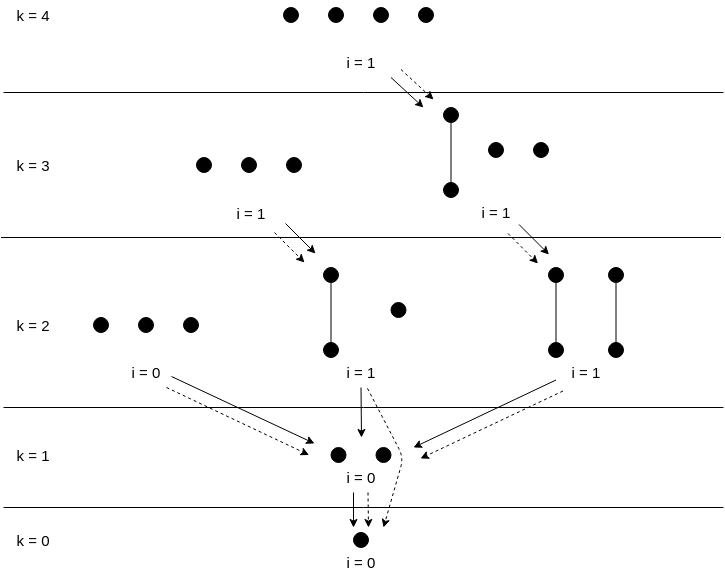
\includegraphics[width=\columnwidth]{figures/backward-search-tree.png}
  \caption{Search tree for $n = 4$ and $i = 1$.
    Level $k$ contains all posets that can be solved in $k$ comparisons and contribute to the solution for the given parameters $n$ and $i$. \\
    Solid arrows indicate predecessors of a poset, while dashed arrows represent the resulting posets when the reversed comparison is inserted.}
  \label{fig:backward-search-tree}
\end{figure}

Figure~\ref{fig:backward-search-tree} illustrates the posets explored in the backward search for $n = 4$ and $i = 1$.

\subsubsection{Normalform} \label{sec:backward:normal_form}
Note that the backward search requires a unique normal form distinct from the pseudo canonified form used in the forward search.
If our custom canonification fails to produce a unique form, nauty provides the appropriate canonified form.
The following outlines the canonification process:

First, determine whether $i < n - 1 - i$ holds.
If not, replace the poset with its dual.
According to Lemma~\ref{lemma:dual_poset_allowed}, the solvability of the poset remains unchanged.

Finally, the posets elements are arranged canonically.
For this purpose, the poset is represented as a directed graph with respect to its Hasse diagram.
The canonic labelling of the elements is provided by nauty, which is a program in \texttt{C} for the calculation of graph automorphism groups \cite[Practical Graph Isomorphism]{MCKAY201494}.
With this canonic labelling the poset can be represented canonically.

A potential issue arises if $i = n - 1 - i$.
In this case, it is impossible to decide whether $P$ or $P^{-1}$ corresponds to the canonical form based on the value of $i$.

\begin{figure}[!b]
  \centering
  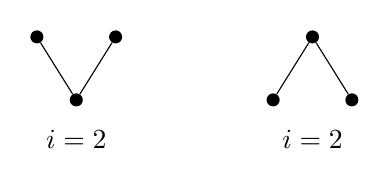
\begin{tikzpicture}
  \node[circle,fill=black,scale=0.5] (A1) at (1, 0) {};
  \node[circle,fill=black,scale=0.5] (A2) at (0.5, 0.8) {};
  \node[circle,fill=black,scale=0.5] (A3) at (1.5, 0.8) {};

  \draw (A1) -- (A2) node {};
  \draw (A1) -- (A3) node {};
  \node (AL) at (1, -0.5) {$i = 2$};


  \node[circle,fill=black,scale=0.5] (B1) at (3 + 1, 0.8) {};
  \node[circle,fill=black,scale=0.5] (B2) at (3 + 0.5, 0) {};
  \node[circle,fill=black,scale=0.5] (B3) at (3 + 1.5, 0) {};

  \draw (B1) -- (B2) node {};
  \draw (B1) -- (B3) node {};
  \node (BL) at (3 + 1, -0.5) {$i = 2$};
\end{tikzpicture}
  \caption{Problematic case where Nauty cannot distinguish between the two posets, despite them being each other's duals. However, according to Lemma~\ref{lemma:dual_poset_allowed} they can be transformed into each other.}
  \label{fig:backward_canonify_problematic}
\end{figure}

In Figure~\ref{fig:backward_canonify_problematic}, the posets as Hasse diagram appear different despite being each other's duals.
To resolve this ambiguity, the dual poset is computed and canonified for each poset where $i = n - 1 - i$ holds true.
Subsequently, one of the posets is deterministically selected.
The deterministic selection is realized by comparing the two binary representations bit by bit.
The representation that first differs by having a '1' is then selected.

Since canonification is inevitable for the backward search but consumes significant computational time, all trivial cases are treated manually and only the remaining cases are canonified by nauty.

The manual canonification works as follows:
First, compute the in- and out-degree for each node.
Then assign a hash value to each node based on these degrees, considering the recursive topological structure of adjacent nodes up to a specified depth limit.

Next, sort the nodes according to their hash values.
If all hash values are unique, the graph finally attains its unique normal form.
For two nodes with identical attributes, it is attempted to swap them.
If the internal representation remains unchanged after swapping, the poset is considered uniquely canonified, since both graphs map to the same internal representation.
If the internal representations differ, the graph is treated as follows:
Let there be $l$ pairs of nodes with identical attributes.
The algorithm iterates through all possible permutations.
E.g. for the first pair, there are two options: either the nodes are swapped or they remain unchanged.
Given the realistic assumption that $l$ is small, all $2^l$ permutations can be efficiently iterated.
With the aim of obtaining values for $n = 15$, it follows that there are at most $7$ pairs, hence $l \leq 7$ always holds.
Finally, one permutation is deterministically selected based on its internal representation, as in the case of the dual poset.

Implementing this canonification preprocessing significantly reduces the number of cases that require nauty, as illustrated in Table~\ref{table:nauty-ratio}.

\begin{table}[!t]
  \renewcommand{\arraystretch}{1.2}
  \caption{Percentage of canonification requiring nauty for variable $n$ and $i$, where lower values are preferable.}
  \label{table:nauty-ratio}
  \centering
  \resizebox{\columnwidth}{!}{%
    \begin{tabular}{c|cccccccc}
      $n$ & \multicolumn{8}{c}{$i$}                                                          \\
          & 0                       & 1      & 2     & 3     & 4     & 5     & 6     & 7     \\ \hline
      13  & 0                       & 30.205 & 6.797 & 1.530 & 0.469 & 0.188 & 0.485 &       \\
      14  & 0                       & 33.667 & 7.540 & 1.655 & 0.427 & 0.153 & 0.074 &       \\
      15  & 0                       & 36.390 & 8.173 & 1.683 & 0.460 & 0.133 & 0.066 & 0.042 \\
    \end{tabular}%
  }
\end{table}

It is particularly noteworthy that as $i$ increases, the percentage of nauty calls decreases.
For small values of $i$, the high percentage of nauty calls is not critical, as computations for small $i$ are generally quick.

\subsubsection{Optimization}

As the theoretical upper bounds are too high in practice, the program uses an iterative deepening approach.
It starts with an upper bound that corresponds to the theoretical lower bound, derived by Lemma~\ref{lemma:previous_next_poset} from the smaller values for $n$ and increases this bound iteratively until a solution is finally found.
As it is not possible to save which posets are lost due to the guessed upper bound without considerable effort, the backward search is restarted several times.
Although results from previous rounds are not used, the search space can be considerably reduced and the program can be made more efficient.

\begin{figure}[!b]
  \centering
  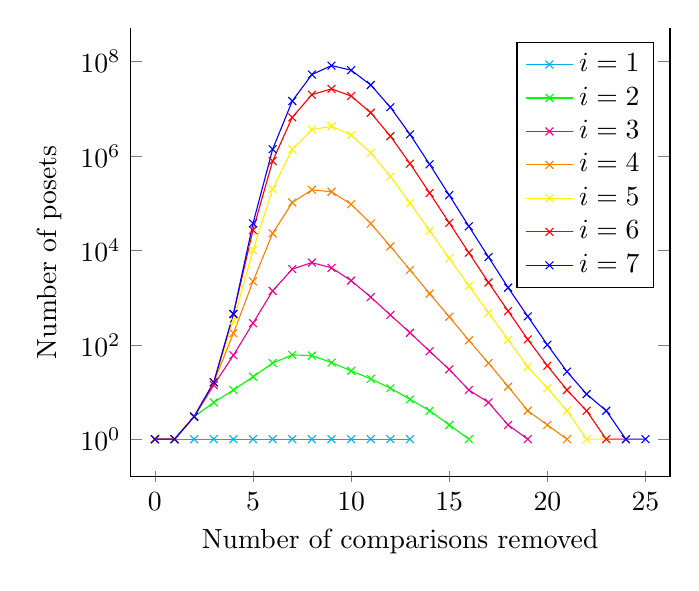
\begin{tikzpicture}
  \begin{axis}[
      ymode=log,
      axis x line = bottom,%x-Achse nur unten
      % x dir=reverse,
      enlarge x limits = .05,%x-Achse erweitern
      x axis line style = {-},%kein Pfeil
      % title = {\dots},
      ylabel={Number of posets},
      xlabel={Number of comparisons removed},
      % only marks,
      cycle list={{mark=x}},
      legend pos=north east,
    ]
    \addlegendentry{$i = 1$}
    \addplot+[cyan] table { %n=14,i=0
        x  y
        0  1
        1  1
        2  1
        3  1
        4  1
        5  1
        6  1
        7  1
        8  1
        9  1
        10 1
        11 1
        12 1
        13 1
      };
    \addlegendentry{$i = 2$}
    \addplot+[green] table { %n=14,i=1
        x y
        0  1
        1  1
        2  3
        3  6
        4  11
        5  21
        6  41
        7  61
        8  59
        9  42
        10 28
        11 19
        12 12
        13 7
        14 4
        15 2
        16 1
      };
    \addlegendentry{$i = 3$}
    \addplot+[magenta] table { %n=14,i=2
        x y
        0  1
        1  1
        2  3
        3  14
        4  60
        5  287
        6  1385
        7  4005
        8  5510
        9  4268
        10 2284
        11 1025
        12 428
        13 180
        14 73
        15 30
        16 11
        17 6
        18 2
        19 1
      };
    \addlegendentry{$i = 4$}
    \addplot+[orange] table { %n=14,i=3
        x y
        0  1
        1  1
        2  3
        3  16
        4  175
        5  2201
        6  22900
        7  103210
        8  191627
        9  174416
        10 94785
        11 37004
        12 12173
        13 3851
        14 1211
        15 392
        16 124
        17 41
        18 13
        19 4
        20 2
        21 1
      };
    \addlegendentry{$i = 5$}
    \addplot+[yellow] table { %n=14,i=4
        x y
        0  1
        1  1
        2  3
        3  16
        4  323
        5  10111
        6  200521
        7  1386176
        8  3607272
        9  4267576
        10 2763862
        11 1162696
        12 367875
        13 100552
        14 26024
        15 6745
        16 1781
        17 474
        18 127
        19 34
        20 12
        21 4
        22 1
        23 1
      };
    \addlegendentry{$i = 6$}
    \addplot+[red] table { %n=14,i=5
        x y
        0  1
        1  1
        2  3
        3  16
        4  446
        5  26921
        6  780123
        7  6588569
        8  19882832
        9  26416869
        10 18631911
        11 8243306
        12 2630332
        13 688904
        14 164372
        15 38334
        16 8918
        17 2084
        18 518
        19 130
        20 36
        21 11
        22 4
        23 1
        24 1
      };
    \addlegendentry{$i = 7$}
    \addplot+[blue] table { % n=14,i=6
        x y
        0  1
        1  1
        2  3
        3  16
        4  452
        5  37236
        6  1389385
        7  14591680
        8  53003482
        9  82198656
        10 65707713
        11 31909980
        12 10770689
        13 2864659
        14 665109
        15 147573
        16 32349
        17 7214
        18 1624
        19 400
        20 100
        21 27
        22 9
        23 4
        24 1
        25 1
      };
  \end{axis}
\end{tikzpicture}
  \caption{Number of posets generated by the backward search for $n = 14$ depending on the number of comparisons for various $i$. Be aware of the logarithmic scale of the y-axis and that the reverse search does not add comparisons, but rather removes them.}
  \label{fig:backward-posets-per-level}
\end{figure}

Figure~\ref{fig:backward-posets-per-level} shows the number of backward search posets for different values of $i$.
It is noticeable that the highest number of posets is searched for all $i$ when there are $8$ to $9$ comparisons left, with a slight tendency towards more comparisons for larger $i$.


\subsubsection{Parallelization} \label{sec:backward:parallelisation}

The backward search can be ideally parallelized by performing the calculation of the predecessors in parallel.
The only two bottlenecks here are read access to the cache and the efficient merging of all partial results.

\begin{table}[!t]
  \renewcommand{\arraystretch}{1.2}
  \caption{Efficiency of parallelism for $n = 13, i = 6$}
  \label{table:backward-parallel}
  \centering
  \begin{tabular}{l|r|l}
    \textbf{number cores} & \textbf{time} & \textbf{efficiency} \\
    \hline
    $1$                   & 7h 2m 59s     & $1.000$             \\
    $2$                   & 3h 57m 9s     & $0.892$             \\
    $4$                   & 2h 41s        & $0.877$             \\
    $8$                   & 1h 2m 9s      & $0.851$             \\
    $16$                  & 32m 57s       & $0.803$             \\
    $32$                  & 20m 11s       & $0.655$             \\
  \end{tabular}
\end{table}

As shown in Table~\ref{table:backward-parallel} for $n = 13$ and $i = 6$, it can be seen that the backward search scales well with the number of cores.
To set the different times in relation to the number of cores, the efficiency was determined, which represents a direct correlation between the two variables.
This can be calculated as follows
\[
  \text{efficiency} = \cfrac{\text{single-core time}}{\text{number of cores} \cdot \text{multi-core time}}
\]
The higher the efficiency, the better the time scales with the number of cores.


\subsection{Bidirectional search} \label{sec:bidirectional}

\subsubsection{Theoretical usability}

In order to enable a bidirectional search, forward and backward searches are combined.
For this purpose, the intersection of the forward and backward search was first determined.

\begin{figure}[!b]
  \centering
  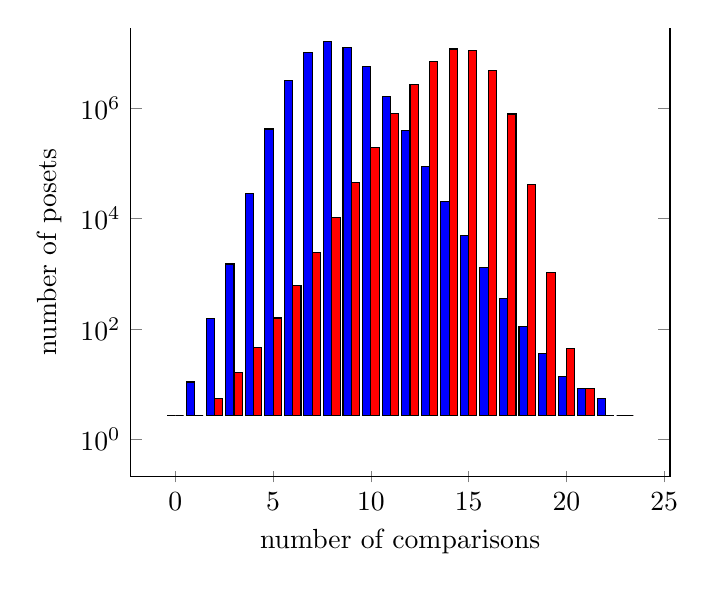
\begin{tikzpicture}
  \begin{axis}[
      ybar,
      ymode=log,
      axis x line = bottom,%x-Achse nur unten
      enlarge x limits = .1,%x-Achse erweitern
      x axis line style = {-},%kein Pfeil
      bar width=3pt,
      ylabel={number of posets},
      xlabel={number of comparisons},
      % legend cell align=left,
      % legend pos=outer north east,
      % legend style={at={(0.5,-0.2)},anchor=north}, % draw=none
    ]
    % \addlegendentry{forward search}
    \addplot[fill=blue,shift={(1pt, 0)}] table {
        x y
        0  1
        1  4
        2  57
        3  552
        4  10397
        5  154828
        6  1166640
        7  3770182
        8  5941732
        9  4726819
        10 2096404
        11 604582
        12 143058
        13 32460
        14 7450
        15 1823
        16 471
        17 132
        18 41
        19 13
        20 5
        21 3
        22 2
        23 1
      };
    % \addlegendentry{backward search}
    \addplot[fill=red,shift={(-1pt, 0)}] table {
        x y
        23 1
        22 1
        21 3
        20 16
        19 381
        18 15227
        17 290138
        16 1750707
        15 4058631
        14 4368185
        13 2592437
        12 1006071
        11 291970
        10 72346
        9  16728
        8  3898
        7  893
        6  227
        5  58
        4  17
        3  6
        2  2
        1  1
        0  1
      };
  \end{axis}
\end{tikzpicture}

Treff: 11
  \caption{Number of posets depending on the number of comparisons for $n = 13$ and $i = 6$ (red: backward search, blue: forward search).}
  \label{fig:backward_forward_count_13_6}
\end{figure}

As shown in Figure~\ref{fig:backward_forward_count_13_6}, the forward search for $n = 13$ and $i = 6$ searches most of the posets with $k = 8$ comparisons, while the backward search searches most of the posets with $k = 14$.

Let's assume that both searches are started in parallel and run until they reach $k = 11$ comparisons.
Due to the logarithmic scaling, this is less noticeable, but the forward search searches from $k = 0$ to $11$ comparisons $99.006\%$ of all posets to be searched in its search space.
Similarly, the backward search searches from $k = 11$ to $23$ comparisons $99.349\%$ of its search space.
This is very unfavorable for a bidirectional search, as there is only a small intersection of both searches.
However, a bidirectional search has been implemented

\subsubsection{Idea}

The idea is to start both searches in parallel and to save the current depth and all posets found up to that point in the backward search in a global variable.
If the forward search goes deeper than the global depth of the backward search, \textit{solvable} is returned if the poset has already been found by the backward search.
Otherwise, \textit{not solvable} is returned.

This approach works because the backward search iterates through all possible posets.
If a poset is not present in the cache of the backward search, it can therefore also not be solvable in the limited number of comparisons.

It should be noted that due to the limited time for the project, the backward search is started with the theoretical upper bound and not the iterative deepening approach is used, as is the case with the pure backward search.
As a result, this is significantly slower than the pure backward search.
Another problem is the internal conversion between the unique canonification of the backward search and the pseudo canonification of the forward search.
For these reasons, the bidirectional search is slower than the pure forward search in the last version of the program.

Nevertheless, bidirectional search has great potential that can be exploited through further research.

% TODO: lemma einbauen

% 2. Zu zeigen: hinzunahem von $u < v$ & reduzieren => Q

% \begin{lemma}
%   Sei $P = (n_P, i_P, R_P)$ ein reduziertes poset.
%   Sei $Q = (n_Q, i_Q, R_Q)$ ein reduziertes poset das man aus $P$ durch hinzufügen eines Vergleichs $u < v$ und anschließendem Reduzieren erhält.
%   Sei $V$ die Menge der Elemente die beim Reduzieren wegfallen mit.
%   Sei $i_Q \leq i_{P'} \leq i_P$.

%   Dann gilt für alle $V' \subseteq V \setminus \{ u, v \}$:
%   Das poset $P' = (n_P - |V'|, i_{P'}, \{ (a, b) \in R_P \mid a, b \notin V' \})$ ist reduziert und durch hinzufügen des Vergleichs $u < v$ und anschließendem Reduzieren erhält man $Q$ aus $P'$.
% \end{lemma}

% \begin{proof}
%   Da $P$ reduziert ist, gilt für jedes Element $x$: $less_P[x] \leq i_P$ und $greater_P[x] \leq n_P - 1 - i_P$

%   Zeige zunächst, dass $P'$ reduziert ist.

%   Für $V' = \emptyset$ gilt $P' = P$ und $P'$ ist somit reduziert.

%   Sei $V' = \{ x \}$.
%   Dann gilt $P' = (n_P - 1, i_{P'}, \{ (a, b) \in R_P \mid a \neq x, b \neq x \})$ mit $i_{P'} \in \{ i_P, (n_P - 1) - 1 - i_P, i_P - 1, (n_P - 1) - 1 - (i_P - 1) \}$.

%   Wenn $i_{P'} = i_P$, dann gilt:
%   \begin{itemize}
%     \item $i_P < n_P - 1 - i_P$ % eig. <=
%     \item für alle Elemente $x$: $less_{P'}[x] \leq less_P[x] \leq i_P \iff less_{P'}[x] \leq i_{P'}$
%     \item für alle Elemente $x$: $greater_{P'}[x] \leq greater_P[x] \leq n_P - 1 - i_P \iff greater_{P'}[x] - 1 \leq (n_{P'} - 1) - 1 - i_{P'}$
%   \end{itemize}

%   Wenn $i_P > n_P - 1 - i_P$:
%   Wenn $i_{P'} = (n_P - 1) - 1 - i_P$, dann $(n_P - 1) - 1 - i_P < i_P$ und somit LESS problematisch


%   Wenn $i_{P'} = i_P - 1$, dann gilt immernoch $n_P - 1 - i_P = (n_P - 1) - 1 - (i_P - 1)$, d.h. greater gleich, aber LESS problematisch

%   Wenn $i_{P'} = (n_P - 1) - 1 - (i_P - 1)$, dann $...$ und somit GREATER problematisch

%   Da nur ein Element entfernt wird, gilt:
%   $less_P'[x] = less_P[x]$ oder $less_P[x] - 1$
%   $greater_P'[x] = greater_P[x]$ oder $greater_P[x] - 1$

%   o.b.d.a gilt $less_P[z] \leq i_P$. Damit Element $z$ wegreduziert werden kann, muss $i_P' < less_P'[z]$ gelten.
%   mit $less_P'[z] = less_P[z]$: $i_{P'} < less_P[z] \leq i_P$. Lösungen: $less_P[z] = i_P$, $less_P[z] = i_P - 1$
%   mit $less_P'[z] = less_P[z] - 1$: $i_{P'} + 1 < less_P[z] \leq i_P$. Lösungen:
%   % D.h. $less_P'[z] = less_P[z]$, also $less_P[z] = i_P' + 1$ und somit $i_P' + 1 = i_P$ => $i_P' = i_P - 1$


%   Weil wir nur Entfernen von Elementen zulassen, die durch das Hinzufügen von $u < v$ rausfliegen, müssen diese in Verbindung mit $u$ oder $v$ stehen.
%   (hier müsste man noch untersuchen unter welchen umständen es dazu kommen kann, dass ein nicht mit denen geordnetes element rausfliegt weil $n$ und $i$ sich durch das entfernen anderer ändern).

%   Damit verändern sich $less$ und $greater$ von $u$ und $v$ parallel zu den $n$ und $i$ von $P$ zu $P'$ und sie sind damit nicht aus $P'$ eliminiert.
%   Andersherum ist zu zeigen dass obwohl die Elemente aus $V \setminus V'$ durch das Entfernen potentiell $less$ und $greater$ verlieren, $n$ und $i$ so verändert sein müssen, dass sie trotzdem rausfliegen.
%   Hier wissen wir, dass alle Elemente kleiner $u$ $greater[v] + 1$ greater dazubekommen haben und das die aus $V$ über die Grenze gebracht hat, umgekehrt für $v$ mit $n_{P'} = n_P - |V'|$ und eventuellen Einschränkungen für $i$ sollte dann begründbar sein, dass sie auch in $P'$ über die Grenze kommen wenn $u < v$. dazukommt
% \end{proof}


\section{Results}

\begin{table}[!t]
  \renewcommand{\arraystretch}{1.2}
  \caption{The minimum number of comparisons needed to select the $i$-th smallest of $n$ elements.}
  \label{table:num-comparisons}
  \centering
  \begin{tabular}{c|cccccccc}
    $n$ & \multicolumn{8}{c}{$i$}                                    \\
        & 0                       & 1  & 2  & 3  & 4  & 5  & 6  & 7  \\ \hline
    1   & 0                                                          \\
    2   & 1                                                          \\
    3   & 2                       & 3                                \\
    4   & 3                       & 4                                \\
    5   & 4                       & 6  & 6                           \\
    6   & 5                       & 7  & 8                           \\
    7   & 6                       & 8  & 10 & 10                     \\
    8   & 7                       & 9  & 11 & 12                     \\
    9   & 8                       & 11 & 12 & 14 & 14                \\
    10  & 9                       & 12 & 14 & 15 & 16                \\
    11  & 10                      & 13 & 15 & 17 & 18 & 18           \\
    12  & 11                      & 14 & 17 & 18 & 19 & 20           \\
    13  & 12                      & 15 & 18 & 20 & 21 & 22 & 23      \\
    14  & 13                      & 16 & 19 & 21 & 23 & 24 & 25      \\
    15  & 14                      & 17 & 20 & 23 & 24 & 26 & 26 & 27 \\
  \end{tabular}
\end{table}

The values we calculated as the minimum number of comparisons needed to solve the selection problem for $n \leq 15$ are shown in Table~\ref{table:num-comparisons}.
For each value we generated an algorithm that solves the problem in that number of comparisons.
We then checked the algorithm on each of the $n!$ permutations to make sure it is correct.

\begin{table}[!t]
  \renewcommand{\arraystretch}{1.2}
  \caption{Execution times of different search methods. Times marked with an asterisk gave a non-optimal result}
  \label{table:search_algorithms}
  \centering
  \begin{tabular}{c|c|l|l|l}
    $n$ & $i$ & \textbf{Forward Search} & \textbf{Backward Search} & \textbf{Oksanen} \\
    \hline
    12  & 0   & 0.0s                    & 0.0s                     & 0.0s             \\
    12  & 1   & 0.0s                    & 0.1s                     & 0.0s             \\
    12  & 2   & 0.4s                    & 0.7s                     & 0.0s             \\
    12  & 3   & 3.5s                    & 1.6s                     & 21.4s*           \\
    12  & 4   & 36.1s                   & 8.4s                     & 4m 59s*          \\
    12  & 5   & 1m 30s                  & 42.0s                    & 1.9s*            \\
    \hline
    13  & 0   & 0.0s                    & 0.0s                     & 0.0s             \\
    13  & 1   & 0.0s                    & 0.5s                     & 0.0s             \\
    13  & 2   & 0.8s                    & 1.5s                     & 0.2s             \\
    13  & 3   & 13.8s                   & 16.1s                    & 55.4s            \\
    13  & 4   & 3m 42s                  & 1m 40s                   & 26m 36s          \\
    13  & 5   & 17m 10s                 & 8m 35s                   & 3h 25m           \\
    13  & 6   & 59m 20s                 & 18m 5s                   & 16h 10m          \\
    \hline
    14  & 0   & 0.0s                    & 0.0s                     & 0.0s             \\
    14  & 1   & 0.0s                    & 1.5s                     & 0.0s             \\
    14  & 2   & 1.4s                    & 5.9s                     & 0.6s             \\
    14  & 3   & 35.9s                   & 46.9s                    & 1m 47s           \\
    14  & 4   & 17m 27s                 & 15m 33s                  & 6h 29m           \\
    14  & 5   & 2h 40m                  & 1h 40m                   & 4d 10h           \\
    14  & 6   & 14h 40m                 & 6h 27m                   & >5d              \\
    \hline
    15  & 0   & 0.0s                    & 0.0s                     & 0.0s             \\
    15  & 1   & 0.1s                    & 4.0s                     & 0.0s             \\
    15  & 2   & 2.8s                    & 25.9s                    & 1.4s             \\
    15  & 3   & 2m 24s                  & 13m 11s                  & 27m 17s          \\
    15  & 4   & 1h 12m                  & 45m 52s                  & 1d 5h 40m        \\
    15  & 5   & 1d 8h 37m               & 19h 30m                  & >5d              \\
    15  & 6   & 4d 23h 37m              & 1d 5h 43m                & >5d              \\
    15  & 7   & 14d 1h 51m              & 3d 8h 9m                 & >5d              \\
  \end{tabular}
\end{table}

Table~\ref{table:search_algorithms} shows the time taken to solve the selection problem.
The times are rounded and may not be representative as the server they were measured on was shared.
The forward search was started with $500$ GB of RAM, and was restarted for each value of $n$ and $i$, so it does not use the cache from previous runs.
The forward search is single-threaded, unlike the backward search, which benefits greatly from parallelism.
The column `Oksanen' shows the times of his program \cite{Oksanen} on our hardware.
Oksanen's program was started with only $25$ GB because it was designed for only $400$ MB RAM.
The numbers marked with an asterisk by Oksanen do not give the optimal lower bound in the publicly available version \texttt{1.6}, even though he has given an optimal algorithm on the website with the unavailable version \texttt{1.1}.

Additionally we measured the number of posets that were stored in the cache after the calculation, which can be seen in Table~\ref{table:cache_entries}.

Furthermore, we can disprove Gasarch's \cite{Gasarch1996} conjecture that ``pair-forming algorithms'', in which the first comparison of any singleton with another singleton is performed, do not lead to suboptimal results.
For $n = 12$ and $i = 4$, this assumption gives a bound of $20$ comparisons, which does not correspond to the optimal bound of $19$ comparisons.

\begin{table}[!t]
  \renewcommand{\arraystretch}{1.2}
  \caption{Number of posets stored in the cache after the corresponding search}
  \label{table:cache_entries}
  \centering
  \begin{tabular}{c|c|r|r}
    $n$ & $i$ & \textbf{Forward Search} & \textbf{Backward Search} \\
    \hline
    13  & 0   & $12$                    & $13$                     \\
    13  & 1   & $329$                   & $245$                    \\
    13  & 2   & $9.7 \cdot 10^3$        & $10.9 \cdot 10^3$        \\
    13  & 3   & $199.7 \cdot 10^3$      & $276.9 \cdot 10^3$       \\
    13  & 4   & $3.7 \cdot 10^6$        & $2.2 \cdot 10^6$         \\
    13  & 5   & $18.1 \cdot 10^6$       & $9.7 \cdot 10^6$         \\
    13  & 6   & $67.6 \cdot 10^6$       & $14.5 \cdot 10^6$        \\
    \hline
    14  & 0   & $13$                    & $14$                     \\
    14  & 1   & $442$                   & $319$                    \\
    14  & 2   & $15.2 \cdot 10^3$       & $19.6 \cdot 10^3$        \\
    14  & 3   & $438.0 \cdot 10^3$      & $644.2 \cdot 10^3$       \\
    14  & 4   & $14.1 \cdot 10^6$       & $13.9 \cdot 10^6$        \\
    14  & 5   & $149.5 \cdot 10^6$      & $84.1 \cdot 10^6$        \\
    14  & 6   & $925.3 \cdot 10^6$      & $263.3 \cdot 10^6$       \\
    \hline
    15  & 0   & $14$                    & $15$                     \\
    15  & 1   & $741$                   & $407$                    \\
    15  & 2   & $23.6 \cdot 10^3$       & $34.9 \cdot 10^3$        \\
    15  & 3   & $1.3 \cdot 10^6$        & $3.1 \cdot 10^6$         \\
    15  & 4   & $53.0 \cdot 10^6$       & $40.0 \cdot 10^6$        \\
    15  & 5   & $1.6 \cdot 10^9$        & $0.73 \cdot 10^9$        \\
    15  & 6   & $5.3 \cdot 10^9$        & $1.3 \cdot 10^9$         \\
    15  & 7   & $15.7 \cdot 10^9$       & $2.2 \cdot 10^9$         \\
  \end{tabular}
\end{table}


\section{Conclusion}

Using computer search based on the work of Oksanen we were able to write our own
version of a search program for selecting the $i$-th element of a list of $n$
elements (see: \href{https://github.com/JGDoerrer/selection_generator}{Github})
and not only confirming the found solutions of Oksanen for the problem but also
improving some entries (e.g. $n = 15, i = 4$). Further we added some more
numbers and therefore algorithms to Table~\ref{table:num-comparisons} for higher $n$ and $i$. As stated
in the motivation before: the road is better than the inn. Along the way we
learned a lot about the problem structure and complexity, improved our forward
and backward search algorithms coming to a final conclusion that both are valid.
If you want to use the program to generate more optimal numbers and therefore
algorithms one should have quite some time and good hardware in form of a high
CPU count and as much RAM as possible (see: \ref{sec:hardware} for our used
hardware).
Right now one should use the backward search due to the lower RAM footprint and
scaling with the CPU count.

Another interesting aspect for the forward search is not only to search for
isomorphic posets in the cache, but also whether a poset is a subgraph of
another. This approach was shortly evaluated, but quickly discarded, since for
each cache lookup the poset to be searched for would have to be compared with
each cache entry, for which the subgraph isomorphism problem, which is
NP-complete, has to be solved each time. Furthermore, this approach only
provides an upper and lower bound for the poset and not an optimal value.

If one is interested in continuing the journey the next steps would be to add
multithreading to the forward search and add the possibility of a bidirectional
search.


\subsection{Used Soft- and Hardware} \label{sec:hardware}

Our results were facilitated by advancements in both hardware and software.
All versions of the software used are listed in the Table~\ref{table:command_outputs}.
For hardware, we employed two Intel Xeon CPUs, each equipped with $12$ cores ($24$ threads), and a total of $768$ GB of RAM.
The latest version of our software can be found on github (\url{https://github.com/JGDoerrer/selection_generator}).

\begin{table}[!t]
  \renewcommand{\arraystretch}{1.2}
  \caption{Specific versions on the software used.}
  \label{table:command_outputs}
  \centering
  \begin{tabular}{l|l}
    \textbf{Command}         & \textbf{Output}                        \\ \hline
    \texttt{rustc -V}        & rustc 1.77.2                           \\ \hline
    \texttt{clang --version} & Ubuntu clang version 14.0.0-1ubuntu1.1 \\ \hline
    \texttt{uname -a}        & Linux plankton 5.15.0-105-generic      \\
  \end{tabular}
\end{table}


\section*{Acknowledgments}

The authors would like to express their appreciation to the FMI for hosting this
research project. Without the provision of their hardware the extensive
computations leading to the attained results would be infeasible. Gratitude is
extended to PD Dr. rer. nat. Armin Weiß for overseeing and grading this project. Special thanks
are due to Florian Stober whose dedicated supervision greatly enriched the
discourse in terms of methodology, implementation and documentation. The
preceded work of PD Dr. rer. nat. Armin Weiß and Florian Stober \textit{Lower Bounds for Sorting
  16, 17, and 18 Elements} \cite{stober2022lower} provided a profound guideline
for the structure of our work.

\ifCLASSOPTIONcaptionsoff
  \newpage
\fi


\bibliographystyle{IEEEtran}
\bibliography{biblio.bib}
\end{document}